\begin{figure}[!htbp]
\centering
\begin{tikzpicture}[schema base,
  priorita/.style={circle,draw=schemaVerde,fill=schemaCartaVerde,font=\schemafont\small\bfseries,inner sep=3pt}]
\node[schema titolo] at (0,0.65) {Testo sorgente: ordine di priorità};
\node[priorita] at (0.1,-0.4) {1};
\pic[scale=0.63] at (1,-1.1) {pagina};
\draw[draw=schemaBlu,line width=1.1pt] (1.1,-0.9) circle (0.25);
\draw[schemaBlu,line width=1.6pt,line cap=round] (1.28,-1.08) -- (1.55,-1.35);
\node[schema etichetta,anchor=west,align=left,text width=4.5cm] at (2,-1.1)
  {\textbf{Riferimenti nella pagina}\\Testo che richiama la figura.};
\node[priorita] at (0.1,-2.75) {2};
\pic[scale=0.63] at (1,-3.45) {documento-strutturato};
\node[schema etichetta,anchor=west,align=left,text width=4.5cm] at (2,-3.45)
  {\textbf{Altrimenti: elementi vicini}\\Nello stesso percorso di capitolo.};
\draw[schema freccia] (1,-1.9) -- node[right,schema nota] {Se assenti} (1,-2.65);
\node[priorita] at (0.1,-5.1) {3};
\pic[scale=0.7] at (1,-5.8) {testo};
\draw[schemaOcra,line width=1.4pt,line cap=round] (0.55,-6.35) -- (1.45,-5.25);
\node[schema etichetta,anchor=west,align=left,text width=4.5cm] at (2,-5.8)
  {\textbf{Se assenti: nessun contesto}\\Né percorso strutturale.};
\draw[schema freccia] (1,-4.25) -- node[right,schema nota] {Se assenti} (1,-5);
\draw[schemaGrigio,line cap=round,line join=round] (6.65,-0.25) -- (7,-0.25) -- (7,-6.5) -- (6.65,-6.5);
\node[schema titolo] at (8.25,0.65) {Richiesta al VLM};
\path[schema pannello,fill=schemaCartaViola!25]
  (8.1,-5.95) -- (8.1,0) -- (10.8,0) -- (11.15,-0.25) -- (15.45,-0.25) -- (15.45,-5.95) -- cycle;
\node[inner sep=0pt] at (9.8,-1.35)
  {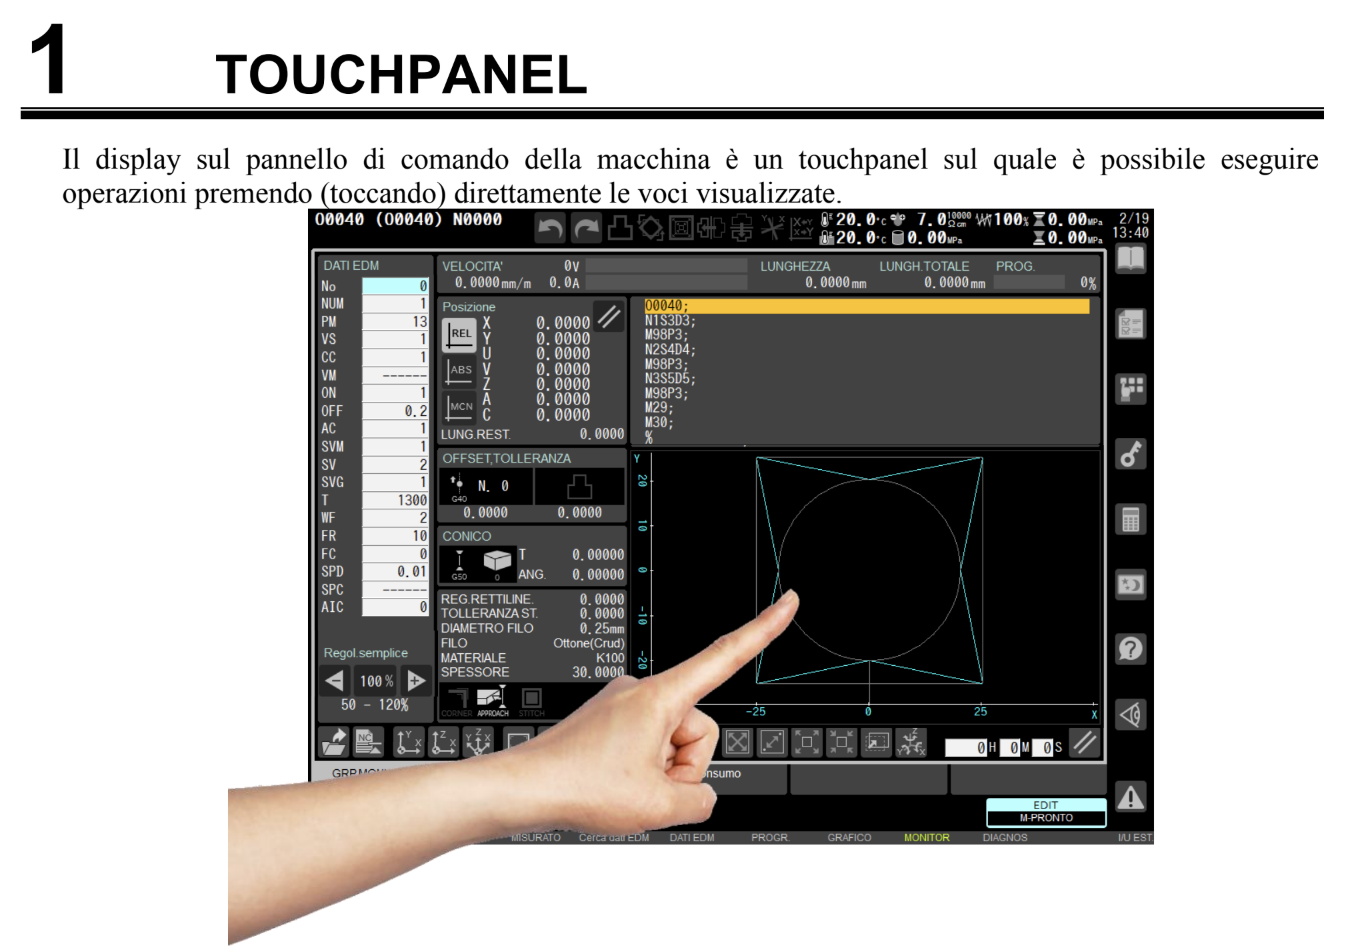
\includegraphics[width=2.5cm,height=1.7cm,keepaspectratio]{figure/asset/touch-panel-schermata-operatore.png}};
\pic[scale=0.7] at (13.25,-1.35) {documento-strutturato};
\node[schema etichetta,text width=2.8cm] at (9.8,-2.7) {\textbf{Ritaglio originale}};
\node[schema etichetta,text width=3.7cm] at (13.25,-2.7)
  {Manuale, pagina ed eventuale caption originale};
\pic[scale=0.67] at (9.4,-4.35) {frammenti};
\node[schema etichetta,text width=3.8cm] at (12.95,-4.35)
  {\textbf{Contesto selezionato}\\Al massimo 6 elementi\\e 2400 caratteri};
\draw[schema freccia] (7,-4.35) -- (8.55,-4.35);
\node[schema nota,text width=6.5cm] at (11.8,-5.45)
  {Il testo serve a disambiguare il visibile.};
\node[schema oggetto,minimum width=2.2cm,minimum height=1.8cm] (vlm) at (9.3,-7.4) {};
\pic[scale=0.8] at (9.3,-7.4) {modello};
\node[schema oggetto,minimum width=2.5cm,minimum height=1.8cm] (descrizione) at (13.1,-7.4) {};
\pic[scale=0.85] at (13.1,-7.4) {dialogo};
\draw[schema freccia] (9.3,-5.95) -- (vlm.north);
\draw[schema freccia] (vlm.east) -- (descrizione.west);
\node[schema etichetta,text width=2.2cm] at (9.3,-8.75) {\textbf{VLM}};
\node[schema etichetta,text width=4.5cm] at (13.1,-8.75)
  {\textbf{Descrizione generata}\\Da confrontare con la fonte};
\pic[scale=0.58] at (0.9,-7.95) {dialogo};
\draw[schemaOcra,line width=1.5pt,line cap=round] (0.25,-8.45) -- (1.55,-7.45);
\node[schema etichetta,anchor=west,align=left,text width=4.8cm] at (2,-8.05)
  {\textbf{Nessun riuso come fonte}\\Le descrizioni generate non entrano nel contesto delle figure successive.};
\end{tikzpicture}
\caption{Composizione degli ingressi del captioning. Le fonti testuali seguono un ordine di priorità, non vengono sommate indiscriminatamente; in assenza di fonti ammissibili, la richiesta non contiene contesto né percorso strutturale. La miniatura dai materiali FANUC forniti è illustrativa, non un risultato del captioning. La descrizione generata va confrontata con la fonte e non diventa una nuova fonte per le richieste successive.}
\label{fig:contesto-caption}
\end{figure}